\documentclass{article}
\usepackage[utf8]{inputenc}
\usepackage{amsmath}
\usepackage{enumitem}
\usepackage{graphicx}
\usepackage{framed}
\usepackage{listings}
\usepackage{pdfpages}
\usepackage{caption}
\usepackage{subcaption}
\usepackage[utf8]{inputenc}
\usepackage{minted}
\usepackage{placeins}
\usepackage[utf8]{inputenc}


\title{Ch 4 Group}
\author{Tate Meehan, Arash Modaresi Rad, William Rudisill}
\date{March 2019}
\begin{document}
\maketitle

\section*{Problem 2.}
\subsection*{a.}
See the attached Matlab code. 

\subsection*{b.}
The bound, $\delta$, reflects the expected difference between the regularized  solution and the true model parameters. Theorem 4.2 in the book provides a bound for the total error from regularization in addition to data noise for a zeroth order Tikonov approximation. The delta value is the amount of noise in the data. Since we have data values accurate to four significant digits, we suppose that a reasonable bound for $\delta$ is within $+/-$ 1E-5. 

\subsection*{Sections c - e}
The alpha values found from the L-curve, discrepancy principle, and GCV methods for the zeroth, first, and second order tikonov solutions.

\begin{table}[ht!]
    \centering
    \begin{tabular}{|c|c|c|c|}
         \hline 
                 & Zeroth & First & Second    \\
         \hline
         L-Curve &  .0340  &  .009 &  .2900   \\ 
         \hline
         Disc. P & 1.54E-6 & 1.54E-6 & 1.41E-6 \\ \hline
         GCV     & 9.77E-4 & -.0068 & -0.0109 \\
         \hline
    \end{tabular}
    \caption{Alpha values for the various experiments}
    \label{tab:my_label}
\end{table}
\vspace{-20pt}
\subsection*{f.}
The solutions for the L0, L1, and L2 solutions cannot be said to be unambiguously real'. The parameters that we have solved for depend on the choice of the roughening matrix. In this case, we are testing the cases where L is a zero order (identity matrix) and first and second order derivatives. So, in this way, we are imposing that our solution should have a certain smoothness. This can be clearly seen in the L1 solution, where the oscillations shown in the zeroth order solution have been smoothed out. The L2 solution still has oscillations, but they have been dampened relative to the zeroth order solution. 

\begin{figure}[ht!]
    \centering
    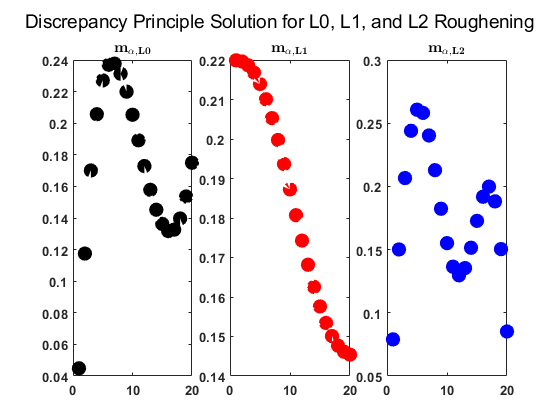
\includegraphics[width=3in]{2f.png}
    \caption{Zeroth Order Tikhonov Solution}
    \label{2fsolutions}
\end{figure}


\section*{Problem 3.}
\subsection*{a.}
Figure \ref{3a1} shows the L curve and the optimal alpha selection for the truncated SVD using two different methods. Figure \ref{3a2} shows the solution for the TSVD problem. For this system, p=3. 

\begin{figure}[ht!]
    \centering
    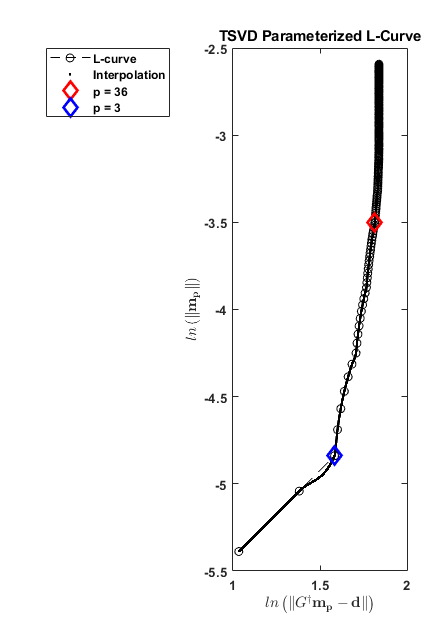
\includegraphics[width=3in]{3a1.png}
    \caption{L-curve. Red diamond uses Borcher's code for selecting optimal $\alpha$. Blue diamonds use Tate's method.}
    \label{3a1}
\end{figure}

\begin{figure}[ht!]
    \centering
    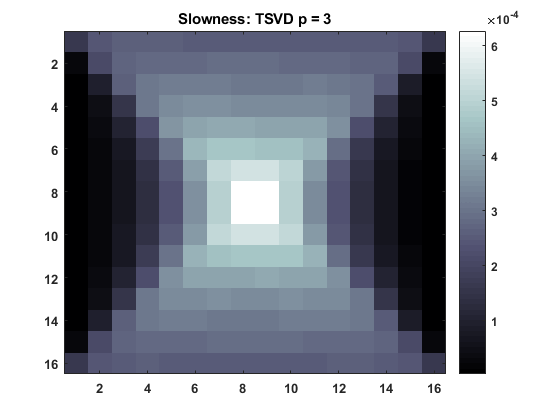
\includegraphics[width=3in]{3a2.png}
    \caption{Solution for the truncated SVD with p=3}
    \label{3a2}
\end{figure}

\FloatBarrier

\subsection*{b.} 
For this problem, the L-curve method is not particularly well suited. This might be because, due to the particular model and the data, the range of the model parameter norm ($\Vert m \Vert$) is quite small compared to the range of the model residual values (Figure \ref{3b1}). Nonetheless, we found an alpha value of $\alpha$ value of 8.8. 
Moreover, it is difficult to select the regularization parameter $\alpha$ using the discrepancy principle because there is no $\chi^2$ for which there is less than one degree of freedom. The degrees of freedom are given by m-n, where m and n are the dimensions of the matrix. A common heuristic is to select m degrees of freedom in this situation. Figure \ref{3b2} shows a solution for the zeroth order Tikhonov. 

\begin{figure}[!h]
    \centering
    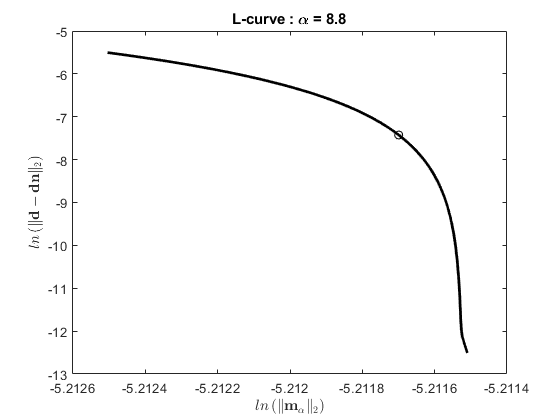
\includegraphics[width=3in]{3b1.png}
    \caption{L-Curve for the zeroth order tikonhov}
    \label{3b1}
\end{figure}

\begin{figure}[!h]
    \centering
    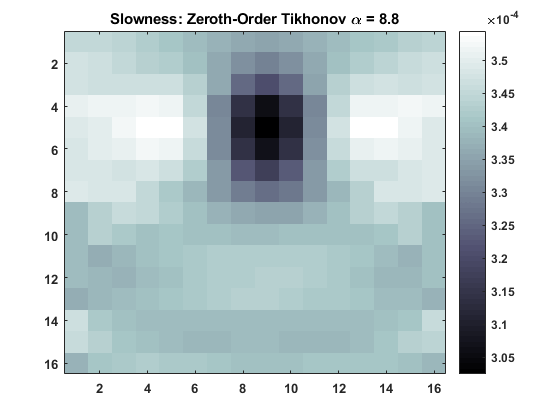
\includegraphics[width=3in]{3b2.png}
    \caption{Solution for the zeroth order tikhonov}
    \label{3b2}
\end{figure}

\FloatBarrier

\subsection*{c.}
A problem does arise when finding the L-curve criterion. We find that the L curve for the second order tikhonov solution is not a monotonic function in the L-curve space (Figure \ref{3c1}). The alpha value that we selected is $\alpha = .7$. Figure \ref{3c2} shows the solution. Again, the L-curve is lacks sensitivity in the image space.

\begin{figure}[!h]
    \centering
    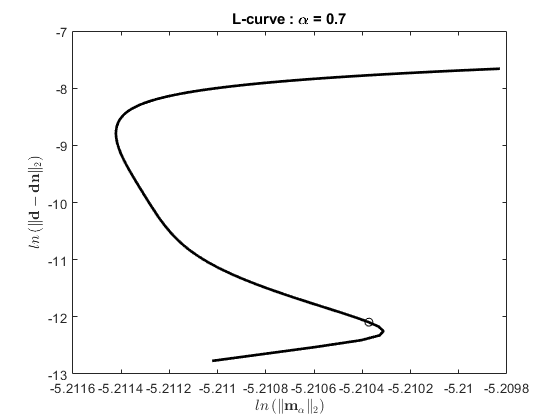
\includegraphics[width=3in]{3c1.png}
    \caption{L Curve for the second order tikhonov}
    \label{3c1}
\end{figure}

\begin{figure}[!h]
    \centering
    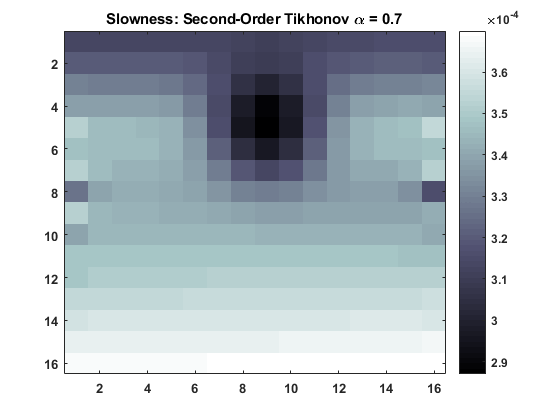
\includegraphics[width=3in]{3c2.png}
    \caption{Second order tikhonov solution}
    \label{3c2}
\end{figure}

\FloatBarrier
\vspace{-20pt}
\subsection*{d.}
We do find that there are vertical stripes on the outside of the domain, going both horizontally and vertically. The values in each row decrease as one moves downwards for the first order Tikhonov solution, but to a lesser extent for the zeroth. The discrepancy is explained by the Laplacian derivative used in the roughening matrix. 



\newpage
\section*{Problem 5.}
The normal equations will satisfy:
\begin{align}
min_m
\Bigg\Vert
\begin{bmatrix}
G \\
\alpha L \\ 
\end{bmatrix}
(m - m_0)
-
\begin{bmatrix}
d \\
0 
\end{bmatrix}
\Bigg\Vert_2^{2}
\end{align}
The normal equations for Equation 1 are then: 

\begin{align}
\begin{bmatrix}
G^T & \alpha L 
\end{bmatrix}
\begin{bmatrix}
G \\
\alpha L 
\end{bmatrix}
(m - m_0)
=
\begin{bmatrix}
G^T & \alpha L 
\end{bmatrix}
\begin{bmatrix}
d \\
0
\end{bmatrix}
\end{align}
Since we know the $m_0$ with which we are seeking to bias the answer, we can solve for m by the following: 
\begin{align}
(G^TG + \alpha L^TL)m = G^Td + (G^TG\alpha^2L^TL)m_0
\end{align}

Letting $Y=X^{-1}$, we can substitute $Yx=m$ and simplify using 4.44 in the book. Likewise, we can let $Yx_0=m_0$ (equivalent to saying $Xm_0 = X_0$). 

\begin{align}
(\lambda^T\lambda + \alpha M^TM)x = \lambda^TU^Td + (\lambda^T\lambda + \alpha M^TM)Xm_0
\end{align}

Since, the left hand side is diagonal, we can solve for $x_i$ by: 

\begin{align}
x_i = \frac{\lambda U^T_{i+k}d + X_{i+k}m_{0,i}}{\lambda_i^2 + \alpha^2\mu_i^2}
\end{align}


\section*{Appendix}
\begin{verbatim}
%% Tate Meehan, Arash Modaresi Rad, Will Rudisill
% Group Assignament Assignment Chapter 4
% clear;close all; clc;
% addpath 'C:\Users\snowfield\Desktop\Backup\Math\Inverse Theory\PEIP-code\Exercises\chap3\prob5';
%load('ifk.mat')
%% Prolem 2 - revisit 3.5
m = length(d);
n = m;
dx = 1./20;
y = dx/2:dx:1;
a = 0;
x = dx/2+((1:20)-1).*dx;
for ii = 1:20
    for jj = 1:20
        g = x(ii).*exp(-(x(ii).*y(jj)));
        G(jj,ii) = g.*dx;
    end
end



% Generalized SVD
%% zeroth - order tikhonov regularization
L = eye(size(G)); 
[U,V,X,Lam,M] = gsvd(G,L);
Y = inv(X)';
% l = sqrt(diag(Lam'*Lam));
% mu = sqrt(diag(M'*M));
% g = l./mu;
% Use fminsearch to solve for the optimal alpha
options = optimset('PlotFcns',@optimplotfval);
fa = @(a)minAlpha(a,Y,Lam,M,U,X,G,d,m);
a0 = 1;
L0alphaGCV = fminsearch(fa,a0,options);

% L-curve
a = 0.001:0.001:2;
for ii = 1:length(a)
    [falpha(ii),tmp1(ii),tmp2(ii)] = minAlphaLcurve(a(ii),Y,Lam,M,U,X,G,d,m);
end
% [reg_corner,ireg_corner,~]=l_curve_corner(tmp1,tmp2,a);
[L0alphaL,L0alphaIx] = maxLcurve(tmp1,tmp2,a);

% Discrepancy Principle
del = @(a)discrepancyPrincipal(a,Y,Lam,M,U,X,G,d,m,L);
a0 = 1;
a1 = 0.0001;
a2 = 100;
[L0alphaDel] = fminbnd(del,a1,a2);
% [deltaL0, L0alphaDel] = fminsearch(del,a0);
a = L0alphaDel;
Gsharp = Y*inv(Lam'*Lam+a.^2*(M'*M))*Lam'*(U'*U)*Lam*X';
maL0 = Gsharp*d;
dcalL0 = Gsharp*maL0;
% 
% figure();plot(tmp1,tmp2,'k','Linewidth',2); hold on
% plot(tmp1(L0alphaIx),tmp2(L0alphaIx),'or','markerfacecolor','r','markersize',7)
% % plot(tmp1(ireg_corner),tmp2(ireg_corner),'or','markerfacecolor','r','markersize',7)
% title(['L-Curve: \alpha = ', num2str(L0alphaL)])
% ylabel('$ln\left(\|\mathbf{m_{\alpha,L}}\|\right)$','interpreter','latex')
% xlabel('$ln\left(\|G^{\sharp}\mathbf{m_{\alpha,L}} - \mathbf{d}\|\right)$','interpreter','latex')
% set(gca,'fontweight','bold')
% 
% figure();plot(a,falpha,'k','linewidth',2); hold on
% plot(a(L0alphaIx),falpha(L0alphaIx),'or','markerfacecolor','r','markersize',7)
% title(['Objective Function: Global Minimum \alpha = ', num2str(L0alphaL)])
% xlabel('$\alpha$','interpreter','latex')
% ylabel('$\frac{m\left\|\mathbf{G} \mathbf{m}_{\alpha , L}-\mathbf{d}\right\|_{2}^{2}}{\mathbf{Tr}\left(\mathbf{I}-\mathbf{G G}^{\sharp}\right)^{2}}$','interpreter','latex')
% set(gca,'fontweight','bold')
% axes('Position',[.6 .6 .25 .25])
% box on
% plot(a(1:10000),falpha(1:10000),'k','linewidth',2); hold on;
% plot(a(313),falpha(313),'or','markerfacecolor','r','markersize',5)
% title('Local Minimum \alpha = 0.0313')
% set(gca,'fontweight','bold')

%% f1rst - order tikhonov regularization
% Build L
L = zeros(m-1,m);
for ii = 1:m-1
    L(ii,ii:ii+1) = [-1,1];
end
[U,V,X,Lam,M] = gsvd(G,L);
Y = inv(X)';
% l = sqrt(diag(Lam'*Lam));
% mu = sqrt(diag(M'*M));
% g = l./mu;
% Use fminsearch to solve for the optimal alpha
options = optimset('PlotFcns',@optimplotfval);
fa = @(a)minAlpha(a,Y,Lam,M,U,X,G,d,m);
a0 = 1;
L1alphaGCV = fminsearch(fa,a0,options);

% L-curve
a = 0.001:0.001:2;
for ii = 1:length(a)
    [falpha(ii),tmp1(ii),tmp2(ii)] = minAlphaLcurve(a(ii),Y,Lam,M,U,X,G,d,m);
end
% [reg_corner,ireg_corner,~]=l_curve_corner(tmp1,tmp2,a);
[L1alphaL,L1alphaIx] = maxLcurve(tmp1,tmp2,a);

% Discrepancy Principle
del = @(a)discrepancyPrincipal(a,Y,Lam,M,U,X,G,d,m,L);
a0 = 1;
a1 = 0.0001;
a2 = 100;
[L1alphaDel] = fminbnd(del,a1,a2);
% Compute the Solution
a = L1alphaDel;
Gsharp = Y*inv(Lam'*Lam+a.^2*(M'*M))*Lam'*(U'*U)*Lam*X';
maL1 = Gsharp*d;
dcalL1 = Gsharp*maL1;
% [deltaL1, L1alphaDel] = fminsearch(del,a0);

%% second - order tikhonov regularization
L = full(gallery('tridiag',n,-1,2,-1));
[U,V,X,Lam,M] = gsvd(G,L);
Y = inv(X)';
% l = sqrt(diag(Lam'*Lam));
% mu = sqrt(diag(M'*M));
% g = l./mu;
% Use fminsearch to solve for the optimal alpha
options = optimset('PlotFcns',@optimplotfval);
fa = @(a)minAlpha(a,Y,Lam,M,U,X,G,d,m);
a0 = 1;
L2alphaGCV = fminsearch(fa,a0,options);

% L-curve
a = 0.001:0.001:2;
for ii = 1:length(a)
    [falpha(ii),tmp1(ii),tmp2(ii)] = minAlphaLcurve(a(ii),Y,Lam,M,U,X,G,d,m);
end
% [reg_corner,ireg_corner,~]=l_curve_corner(tmp1,tmp2,a);
[L2alphaL,L2alphaIx] = maxLcurve(tmp1,tmp2,a);

% Discrepancy Principle
del = @(a)discrepancyPrincipal(a,Y,Lam,M,U,X,G,d,m,L);
a0 = 1;
a1 = 0.0001;
a2 = 100;
% [deltaL2, L2alphaDel] = fminsearch(del,a0);
[L2alphaDel] = fminbnd(del,a1,a2);

% Compute the Solution
a = L1alphaDel;
Gsharp = Y*inv(Lam'*Lam+a.^2*(M'*M))*Lam'*(U'*U)*Lam*X';
maL2 = Gsharp*d;
dcalL2 = Gsharp*maL2;

figure();plot(x,d); hold on; plot(x,dcalL0);plot(x,dcalL1);plot(x,dcalL2)
legend('data','L0','L1','L2')
%% Plot The solutions from the discrepancy principle
figure(); 
subplot(1,3,1)
plot(1:length(maL0),maL0,'ok','markerfacecolor','k','markersize',10)
title('$\mathbf{m_{\alpha ,L0}}$','interpreter','latex')
set(gca,'fontweight','bold')
subplot(1,3,2)
plot(1:length(maL1),maL1,'or','markerfacecolor','r','markersize',10)
title('$\mathbf{m_{\alpha ,L1}}$','interpreter','latex')
set(gca,'fontweight','bold')
subplot(1,3,3)
plot(1:length(maL2),maL2,'ob','markerfacecolor','b','markersize',10)
title('$\mathbf{m_{\alpha ,L2}}$','interpreter','latex')
set(gca,'fontweight','bold')
suptitle('Discrepancy Principle Solution for L0, L1, and L2 Roughening') 
%%
function [falpha] = minAlpha(a,Y,Lam,M,U,X,G,d,m)
Gsharp = Y*inv(Lam'*Lam+a.^2*(M'*M))*Lam'*(U'*U)*Lam*X';
maL = Gsharp*d;
falpha = (m*norm(G*maL-d).*2)/(trace(eye(m)-G*Gsharp).^2);
end

function [falpha,tmp1,tmp2] = minAlphaLcurve(a,Y,Lam,M,U,X,G,d,m)
Gsharp = Y*inv(Lam'*Lam+a.^2*(M'*M))*Lam'*(U'*U)*Lam*X';
maL = Gsharp*d;
falpha = (m*norm(G*maL-d).*2)/(trace(eye(m)-G*Gsharp).^2);
tmp1 = log(norm(G*maL-d));
tmp2 = log(norm(maL));
end

function [discrepancy] = discrepancyPrincipal(a,Y,Lam,M,U,X,G,d,m,L)
Gsharp = Y*inv(Lam'*Lam+a.^2*(M'*M))*Lam'*(U'*U)*Lam*X';
mp = Gsharp*d;
discrepancy = norm(G*mp - d).^2 + a.^2*norm(L*mp).^2 - m;
end

function [bestAlpha,Kmax] = maxLcurve(tmp1,tmp2,alph)
% tmp1 = log(norm(Gm-d))
% tmp2 = log(norm(m))
% alph = array of alphas used to generate tmp1 and tmp2
 % Interpolate L-curve
 vx = linspace(min(tmp1),max(tmp1),length(alph));
 h = mean(diff(vx));
 L = pchip(tmp1,tmp2,vx);
 clear ('L1','L2')
 aLph = linspace(min(alph),max(alph),length(L));

 % Calculate Curvature
% Better Derivatives
for ii= 3:length(L)-2
L1(ii) = ((L(ii+2) - L(ii-2)) - 8*(L(ii+1) - L(ii-1)))/(12.*h);
end
L1(1:2) = [];
% L1([1:2,end-1:end]) = [];
for ii= 3:length(L1)-2
L2(ii) = ((L1(ii+2) - L1(ii-2)) - 8*(L1(ii+1) - L1(ii-1)))/(12.*h);
end
L2(1:2) = [];
% L2([1:2,end-1:end]) = [];
% Extract The Valid Indices
diffix = (length(L) - length(L2))./2;
L([1:diffix,length(L)-diffix+1:end]) = [];
diffix = (length(L1) - length(L2))./2;
L1([1:diffix,length(L1)-diffix+1:end]) = [];

 K = abs(L2)./(1+L1.^2).^(3/2);
 % median filter
%  K = medfilt1(K,151);
 % Maximize Curvature to find alpha
 [~,Kmax] = max(K);
 
alphix = (length(aLph) - length(L))./2;
aLph([1:alphix,length(vx)-alphix+1:end]) = [];
vx([1:alphix,length(vx)-alphix+1:end]) = [];
bestAlpha = (aLph(Kmax));
end

function hout=suptitle(str)
%SUPTITLE puts a title above all subplots.
%
%	SUPTITLE('text') adds text to the top of the figure
%	above all subplots (a "super title"). Use this function
%	after all subplot commands.
%
%   SUPTITLE is a helper function for yeastdemo.

%   Copyright 2003-2010 The MathWorks, Inc.


% Warning: If the figure or axis units are non-default, this
% will break.

% Parameters used to position the supertitle.

% Amount of the figure window devoted to subplots
plotregion = .92;

% Y position of title in normalized coordinates
titleypos  = .95;

% Fontsize for supertitle
fs = get(gcf,'defaultaxesfontsize')+4;

% Fudge factor to adjust y spacing between subplots
fudge=1;

haold = gca;
figunits = get(gcf,'units');

% Get the (approximate) difference between full height (plot + title
% + xlabel) and bounding rectangle.

if (~strcmp(figunits,'pixels')),
    set(gcf,'units','pixels');
    pos = get(gcf,'position');
    set(gcf,'units',figunits);
else
    pos = get(gcf,'position');
end
ff = (fs-4)*1.27*5/pos(4)*fudge;

% The 5 here reflects about 3 characters of height below
% an axis and 2 above. 1.27 is pixels per point.

% Determine the bounding rectangle for all the plots

% h = findobj('Type','axes');

% findobj is a 4.2 thing.. if you don't have 4.2 comment out
% the next line and uncomment the following block.

h = findobj(gcf,'Type','axes');  % Change suggested by Stacy J. Hills

max_y=0;
min_y=1;
oldtitle = NaN;
numAxes = length(h);
thePositions = zeros(numAxes,4);
for i=1:numAxes
    pos=get(h(i),'pos');
    thePositions(i,:) = pos;
    if (~strcmp(get(h(i),'Tag'),'suptitle')),
        if (pos(2) < min_y)
            min_y=pos(2)-ff/5*3;
        end;
        if (pos(4)+pos(2) > max_y)
            max_y=pos(4)+pos(2)+ff/5*2;
        end;
    else
        oldtitle = h(i);
    end
end

if max_y > plotregion,
    scale = (plotregion-min_y)/(max_y-min_y);
    for i=1:numAxes
        pos = thePositions(i,:);
        pos(2) = (pos(2)-min_y)*scale+min_y;
        pos(4) = pos(4)*scale-(1-scale)*ff/5*3;
        set(h(i),'position',pos);
    end
end

np = get(gcf,'nextplot');
set(gcf,'nextplot','add');
if ishghandle(oldtitle)
    delete(oldtitle);
end
axes('pos',[0 1 1 1],'visible','off','Tag','suptitle');
ht=text(.5,titleypos-1,str);set(ht,'horizontalalignment','center','fontsize',fs);
set(gcf,'nextplot',np);
axes(haold); %#ok<MAXES>
if nargout,
    hout=ht;
end


end

%% Chapter 4 Group Assignment Question 3
clear; close all; clc;

addpath 'C:\Users\snowfield\Desktop\Backup\Math\Inverse Theory\PEIP-code\Lib'
addpath 'C:\Users\snowfield\Desktop\Backup\Math\Inverse Theory\PEIP-code\Exercises\chap4\prob2'
addpath 'C:\Users\snowfield\Desktop\Backup\Math\Inverse Theory\PEIP-code\Exercises\chap4\prob3'

%% Load the Crosswell Data
load('crosswell.mat')
% %% a. Use TSVD
[m,n] = size(G);
p = rank(G);
p = 3;
[U,S,V] = svd(G);
s = diag(S);
Up = U(:,1:p);
Sp = S(1:p,1:p);
sp = diag(Sp);
sp = 1./(sp(:));
Vp = V(:,1:p);
Gdag = (Vp.*sp.')*Up';
% Gdag = Vp.*(sp)'*Up';
mdag = Gdag*dn;
slowness = reshape(mdag,16,16)';

% L-curve method
% Alpha
% q = 1:n;
q = 1:200;
% ma
for kk = 1:length(q)
ma = zeros(n,p);
% Compute filter factors
% f = s.^2./(s.^2+alpha(kk).^2);
for ii = 1:kk
ma(:,ii) = ((U(:,ii)'*dn)./s(ii))*V(:,ii);
end
ma = sum(ma,2);
mq(:,kk) = ma;
normq(kk) = norm(mq);
d = G*mq;
r = norm(d-dn);
normR(kk) = r; 
end

%%
[q_corner, ~, ~] = l_curve_corner(normR, normq, q);
% By inspection q_corner = 85
q_corn = 85;
% plot(log(normR(q_corner)),log(normq(q_corner)),'ob','markersize',10,'markerfacecolor','b')
m85 = mq(:,q_corn);
m85 = reshape(m85,16,16)';

% Interpolate L-curve
 vx = linspace(min(log(normR(:))),max(log(normR(:))),2000);
%  vx = logspace(min(log(normR(:))),max(log(normR(:))),200);
 h = mean(diff(vx));
%  h = mean(diff(log(vx)));

%  L = lagrangePoly(tmp,tmp2,vx);
 L = pchip(log(normR(:)),log(normq(:)),vx);
 aLph = linspace(1,max(q),length(L));
%  aLph = logspace(1,max(q),length(L));

 % Borcher
 [q_borcher, ~, ~] = l_curve_corner(exp(vx), exp(L), aLph);
%  figure();
%  plot(vx,L,'.k');hold on; plot(vx(q_borcher),L(q_borcher),'ok')
 % Calculate Curvature
% Better Derivatives
for ii= 3:length(L)-2
L1(ii) = ((L(ii+2) - L(ii-2)) - 8*(L(ii+1) - L(ii-1)))/(12.*h);
end
L1(1:2) = [];
% L1([1:2,end-1:end]) = [];
for ii= 3:length(L1)-2
L2(ii) = ((L1(ii+2) - L1(ii-2)) - 8*(L1(ii+1) - L1(ii-1)))/(12.*h);
end
L2(1:2) = [];
% L2([1:2,end-1:end]) = [];
% Extract The Valid Indices
diffix = (length(L) - length(L2))./2;
L([1:diffix,length(L)-diffix+1:end]) = [];
diffix = (length(L1) - length(L2))./2;
L1([1:diffix,length(L1)-diffix+1:end]) = [];

 K = abs(L2)./(1+L1.^2).^(3/2);
 % median filter
%  K = medfilt1(K,151);
 % Maximize Curvature to find alpha
 [~,Kmax] = max(K);
 
 alphix = (length(aLph) - length(L))./2;
aLph([1:alphix,length(vx)-alphix+1:end]) = [];
vx([1:alphix,length(vx)-alphix+1:end]) = [];
 bestAlpha = (aLph(Kmax));
 
 %%% Plot L-Curve
 figure();
plot(log(normR),log(normq),'--ok'); hold on
plot(vx,L,'.k','linewidth',2);
% plot(log(normR(q_corn)),log(normq(q_corn)),'ob','markersize',10)
plot(log(normR(q_corner)),log(normq(q_corner)),'dr','linewidth',2,'markersize',10)%,'markerfacecolor','r')
hold on; plot((vx(Kmax)),(L(Kmax)),'db','linewidth',2,'markersize',10)%,'markerfacecolor','b')
title('TSVD Parameterized L-Curve')
ylabel('$ln\left(\|\mathbf{m_{p}}\|\right)$','interpreter','latex')
xlabel('$ln\left(\|G^{\dagger}\mathbf{m_{p}} - \mathbf{d}\|\right)$','interpreter','latex')
legend('L-curve','Interpolation','p = 36','p = 3','location','northwestoutside')
daspect([1 1 1])
set(gca,'fontweight','bold')

figure();imagesc(slowness);colormap(bone);colorbar
title('Slowness: TSVD p = 3')
set(gca,'fontweight','bold')

%% b. zeroth - order tikhonov
% b. Use zeroth-order Tikonov Regularization
 I = eye(m);
 alph = 0.1:0.1:25;
 for ii = 1:length(alph)
 mtik(:,ii) = (G'*G+alph(ii).^2*I)\G'*dn;%G'*inv(G*G'+alph(ii).^2*I)*dn;
 tmp1(ii) = log(norm(mtik(:,ii)));
 d = G*mtik(:,ii);
 tmp2(ii) = log(norm(d-dn));
 end
 
 % Interpolate L-curve
 vx = linspace(min(tmp1),max(tmp1),length(alph));
 h = mean(diff(vx));
 L = pchip(tmp1,tmp2,vx);
 clear ('L1','L2')
 aLph = linspace(min(alph),max(alph),length(L));

 % Calculate Curvature
% Better Derivatives
for ii= 3:length(L)-2
L1(ii) = ((L(ii+2) - L(ii-2)) - 8*(L(ii+1) - L(ii-1)))/(12.*h);
end
L1(1:2) = [];
% L1([1:2,end-1:end]) = [];
for ii= 3:length(L1)-2
L2(ii) = ((L1(ii+2) - L1(ii-2)) - 8*(L1(ii+1) - L1(ii-1)))/(12.*h);
end
L2(1:2) = [];
% L2([1:2,end-1:end]) = [];
% Extract The Valid Indices
diffix = (length(L) - length(L2))./2;
L([1:diffix,length(L)-diffix+1:end]) = [];
diffix = (length(L1) - length(L2))./2;
L1([1:diffix,length(L1)-diffix+1:end]) = [];

 K = abs(L2)./(1+L1.^2).^(3/2);
 % median filter
%  K = medfilt1(K,151);
 % Maximize Curvature to find alpha
 [~,Kmax] = max(K);
 
 figure();plot(K)
 alphix = (length(aLph) - length(L))./2;
aLph([1:alphix,length(vx)-alphix+1:end]) = [];
vx([1:alphix,length(vx)-alphix+1:end]) = [];
 bestAlpha = (aLph(Kmax));
 
 % by inspection
 Kmax = 88;
 bestAlpha = 8.8;
 
 slowness = mtik(:,Kmax);
 slowness = reshape(slowness,16,16)';
 figure();imagesc(slowness);colormap(bone);colorbar
title(['Slowness: Zeroth-Order Tikhonov \alpha = ',num2str(bestAlpha)])
set(gca,'fontweight','bold')
 
 figure();plot(tmp1,tmp2,'k','linewidth',2);
 hold on; plot(tmp1(Kmax),tmp2(Kmax),'ok')
 xlabel('$ln\left(\|\mathbf{m}_\alpha\|_2\right)$','interpreter','latex')
 ylabel('$ln\left(\|\mathbf{d} - \mathbf{dn}\|_2\right)$','interpreter','latex')
 title(['L-curve : \alpha = ',num2str(bestAlpha)])%,'interpreter','latex')
 
 %% c. second order tikhonov regularization
 L=zeros(14*14,256);
 k=1;
 for i=2:15
     for j=2:15
         M=zeros(16,16);
         M(i,j)=-4;
         M(i,j+1)=1;
         M(i,j-1)=1;
         M(i+1,j)=1;
         M(i-1,j)=1;
         L(k,:)=reshape(M,256,1)';
         k=k+1;
     end
 end
 
  alph = 0.1:0.1:25;
 for ii = 1:length(alph)
 mtik(:,ii) = (G'*G+alph(ii).^2*L'*L)\G'*dn;%G'*inv(G*G'+alph(ii).^2*I)*dn;
 tmp1(ii) = log(norm(mtik(:,ii)));
 d = G*mtik(:,ii);
 tmp2(ii) = log(norm(d-dn));
 end
 
 [reg_corner, ~, ~] = l_curve_corner(exp(tmp1), exp(tmp2), alph)
 
 % Interpolate L-curve
 vx = linspace(min(tmp1),max(tmp1),length(alph));
 h = mean(diff(vx));
 L = pchip(tmp1,tmp2,vx);
 aLph = linspace(min(alph),max(alph),length(L));
 clear ('L1','L2')

 % Calculate Curvature
% Better Derivatives
for ii= 3:length(L)-2
L1(ii) = ((L(ii+2) - L(ii-2)) - 8*(L(ii+1) - L(ii-1)))/(12.*h);
end
L1(1:2) = [];
% L1([1:2,end-1:end]) = [];
for ii= 3:length(L1)-2
L2(ii) = ((L1(ii+2) - L1(ii-2)) - 8*(L1(ii+1) - L1(ii-1)))/(12.*h);
end
L2(1:2) = [];
% L2([1:2,end-1:end]) = [];
% Extract The Valid Indices
diffix = (length(L) - length(L2))./2;
L([1:diffix,length(L)-diffix+1:end]) = [];
diffix = (length(L1) - length(L2))./2;
L1([1:diffix,length(L1)-diffix+1:end]) = [];

 K = abs(L2)./(1+L1.^2).^(3/2);
 % median filter
%  K = medfilt1(K,151);
 % Maximize Curvature to find alpha
 [~,Kmax] = max(K);
 
 alphix = (length(aLph) - length(L))./2;
aLph([1:alphix,length(vx)-alphix+1:end]) = [];
vx([1:alphix,length(vx)-alphix+1:end]) = [];
 bestAlpha = (aLph(Kmax));
 
 %By inspection
 Kmax = 7;
 bestAlpha = 0.7;
 
 slowness = mtik(:,Kmax);
 slowness = reshape(slowness,16,16)';
 figure();imagesc(slowness);colormap(bone);colorbar
title(['Slowness: Second-Order Tikhonov \alpha = ',num2str(bestAlpha)])
set(gca,'fontweight','bold')
 
 figure();plot(tmp1,tmp2,'k','linewidth',2);
 hold on; plot(tmp1(Kmax),tmp2(Kmax),'ok')
 xlabel('$ln\left(\|\mathbf{m}_\alpha\|_2\right)$','interpreter','latex')
 ylabel('$ln\left(\|\mathbf{d} - \mathbf{dn}\|_2\right)$','interpreter','latex')
 title(['L-curve : \alpha = ',num2str(bestAlpha)])%,'interpreter','latex')
\end{verbatim}
\end{document}
